\chapter{Related work}


\todo[inline]{mention here rhyme generating tools like rhymezone, redddy also mentions generation}
\section{Rhyme detection tools}
\todo[inline]{Pridat nejaky nastroj co pouziva len CMU dictionary}
\subsection{SPARSAR}


\subsection{Unsupervised approach}
\subsubsection*{EM algorithm}
\cite{reddy2011unsupervised} proposed a language-independent model for finding rhyme schemes in poetry. They created an unsupervised model based on EM algorithm that assigns the most probable rhyme scheme for each sequence of line-end words. It achieved good results when tested on annotated English and French corpus with poetry from 15\textsuperscript{th} to 20\textsuperscript{th} century. However its big pitfall lies in the fact that it is biased towards the rhyme schemes from golden data. It has a predefined set of all rhyme schemes found in tested data and those are the only ones it chooses from. For illustration, in 14-line stanza it can choose from 90 schemes which is only 0.00005\% of all possible options. In 29\% of cases from French corpus it has only one choice.

\subsubsection*{RhymeTagger}
\cite{plechavc2018collocation} came with a collocation-driven alternative named RhymeTagger. It uses the same dataset as previous approach with addition of a larger Czech poetry corpus. Each line-end word is transcribed into phonetic transcription and split into components (syllable peaks and consonant clusters). Probabilities for each component pair are calculated based on their vertical co-occurrence in line-end words. If two words have joined probability for all their components above the set threshold they are considered a rhyme. After all such pairs are classified, probabilities are iteratively recalculated. For words that were not successfully classified with this method, there is a fallback. The author observed that some words changed pronunciation over time and some didn't. Prior pronunciation can be therefore inferred from words with similar orthography. He calculated rhyme probability given character trigrams which helped achieve higher recall as seen in \ref{screenshotRT}.

\begin{figure}[h]\centering
	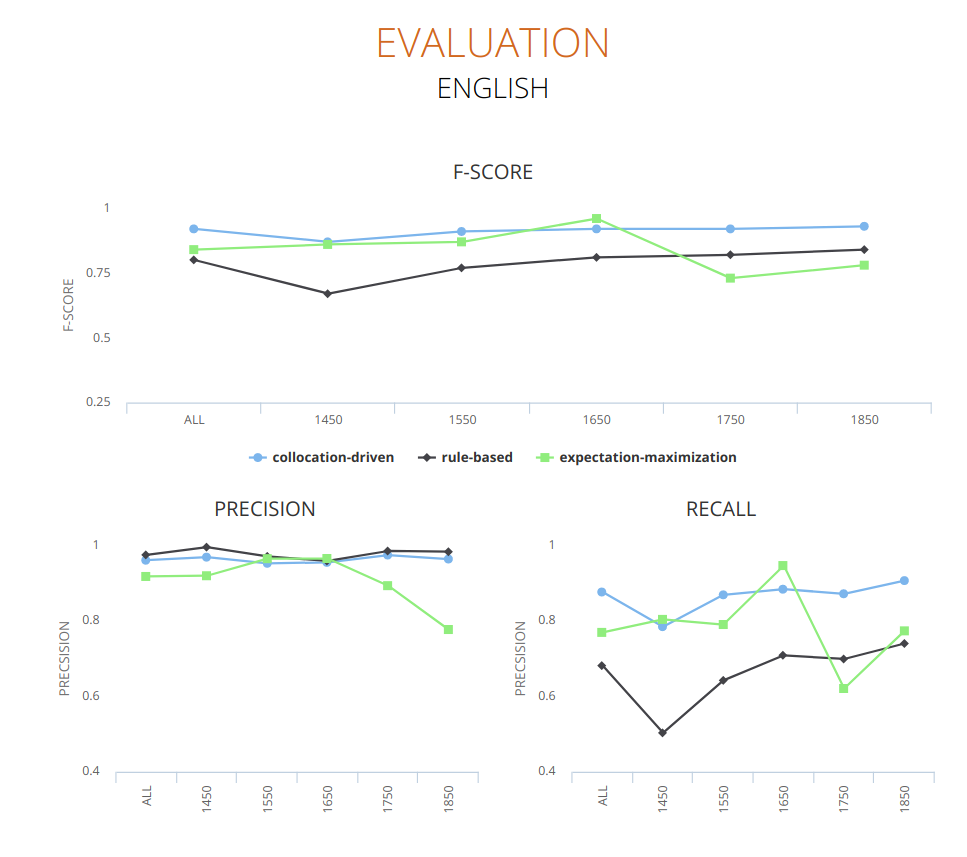
\includegraphics[scale=0.4]{../img/plechac_eval.png}
	\caption{Evaluation of RhymeTagger on English corpus in comparison with EM algorithm and simple rule-based approach.\protect\footnote{http://versologie.cz/talks/2017basel/evaluation\_en.php?lang=en}}\label{screenshotRT}
\end{figure}

\subsubsection*{Deep-speare}
As a part of their sonnet quatrain generating model, \cite{lau2018deep} have a Rhyme component that identifies and generates rhymes. It is a unidirectional forward LSTM that learns to separate rhyming word pairs from non-rhyming. They generate input by pairing one line-end word with the other three from the same quatrain what results in one rhyming pair and two non-rhyming. Additional non-rhyming pairs are generated with random word sampling. Then the model with margin-based loss learns the margin separating the best pair from all the others. It returns a cosine similarity score that estimates how well do two words rhyme.

To evaluate this model, authors used phoneme matching with CMU dictionary \footnote{http://www.speech.cs.cmu.edu/cgi-bin/cmudict} and the EM model from \cite{reddy2011unsupervised} trained on their own data and they were able to outperform both based on F1 score.



\section{Visualization tools}
In the following section we will describe existing visualization tools for poetry. There is no specific software for analyzing song lyrics in particular since they can be considered just a more structurally relaxed version of a regular poem.
\subsection{Poem Viewer}
The most complex and comprehensive visualization tool is Poem Viewer \cite{Abdul2013}. With no need for complicated installations it is easily available for the writers as a web-based application as shown in Figure \ref{screenshotPV}. Unfortunately, at the time of writing this thesis the upload of custom text was not working. Luckily, this is still an ongoing project so this might be just a temporary issue. Nevertheless there are some default poems available to demonstrate this software's capabilities.
\begin{figure}[h]\centering
	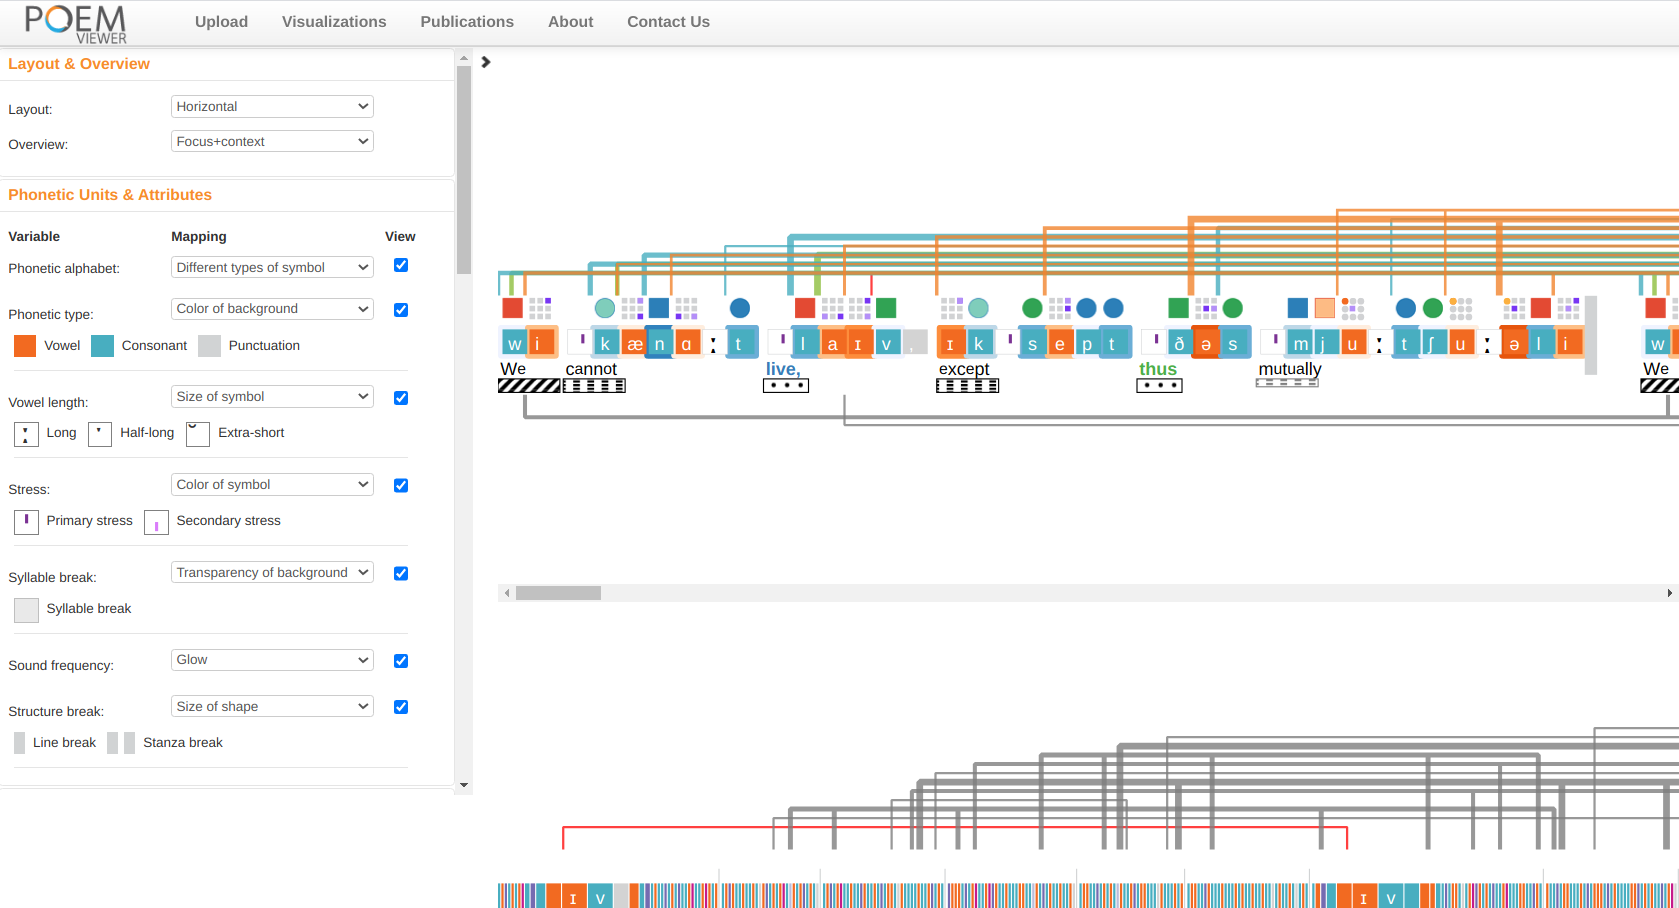
\includegraphics[scale=0.24]{../img/ScreenshotPV.png}
	\caption{Screenshot from Poem Viewer tool - visualizing Love by Elizabeth Barrett Browning.}\label{screenshotPV}
\end{figure}

\begin{figure}[h]\centering
	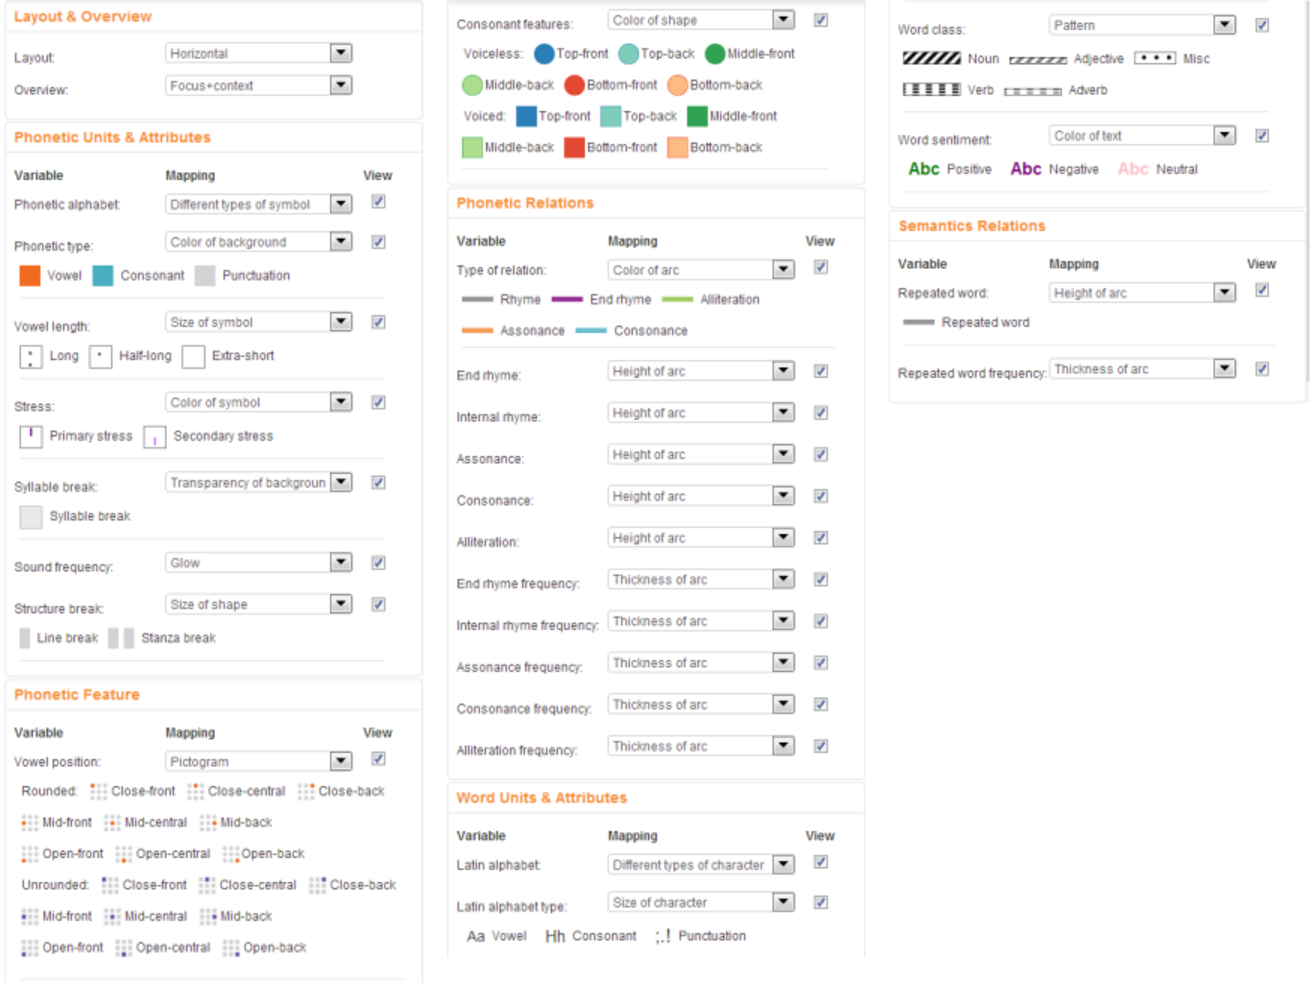
\includegraphics[scale=0.4]{../img/snapshotPV_options.pdf}
	\caption{Available options and their default mappings in Poem Viewer.}\label{screenshotPV-options}
\end{figure}

Most of the analyzed features (shown in Figure \ref{screenshotPV-options} focuses on the phonetic aspects of the poem. After phonetic transcription to IPA users can analyze consonant features, vowel length and position, stress, syllables, word classes and sentiment using color codes and markers. A second layout offers six different graphs/animations of tongue positions during each verse. Arcs are used to mark end rhyme, alliteration, assonance, consonance, their particular frequencies and repeating words.


Overall this software, although very elaborate, appears crowded and confusing for an inexperienced user. It is perhaps better suited for its original use case - a well structured poem - than less regular song lyrics.

\subsection{SPARSAR}
SPARSAR (\cite{Delmonte2014}) is also a very interesting tool for poetry analysis and expressive Text-to-speech conversion. It is originally designed for a thorough examination of a very strictly structured Shakespeare's sonnets. To achieve this, it has to run analyses on many levels - and these results can be used to analyze any poem. It looks at the poem on three views: phonetic (pronunciation, consonant and vowel tongue position, assonances, etc.), poetic (metrical structure, rhyme schemes, acoustic length, etc.), and semantic (sentiment, methaphorically linked words, anaphora, etc.).

User can choose between a window application with graphs and diagrams or a headless mode with .xml output files. Its main disadvantage for our usecase is that it's written in Prolog and therefore is very strict on the input format and runs only under a specific older version of Ubuntu. 

\subsection{ProseVis}
This Java desktop visualization tool by \cite{Clement2013} analyzes text through
parts-of-speech, accent, phoneme, stress, tone, and break index. These features are extracted using OpenMary Text-to-speech system (\cite{Schroder2006}) and predictive classification. The authors believe their visualization will present the features to user in a more human readable form \footnote{https://sourceforge.net/projects/prosevis/}.

\begin{figure}[h]\centering
	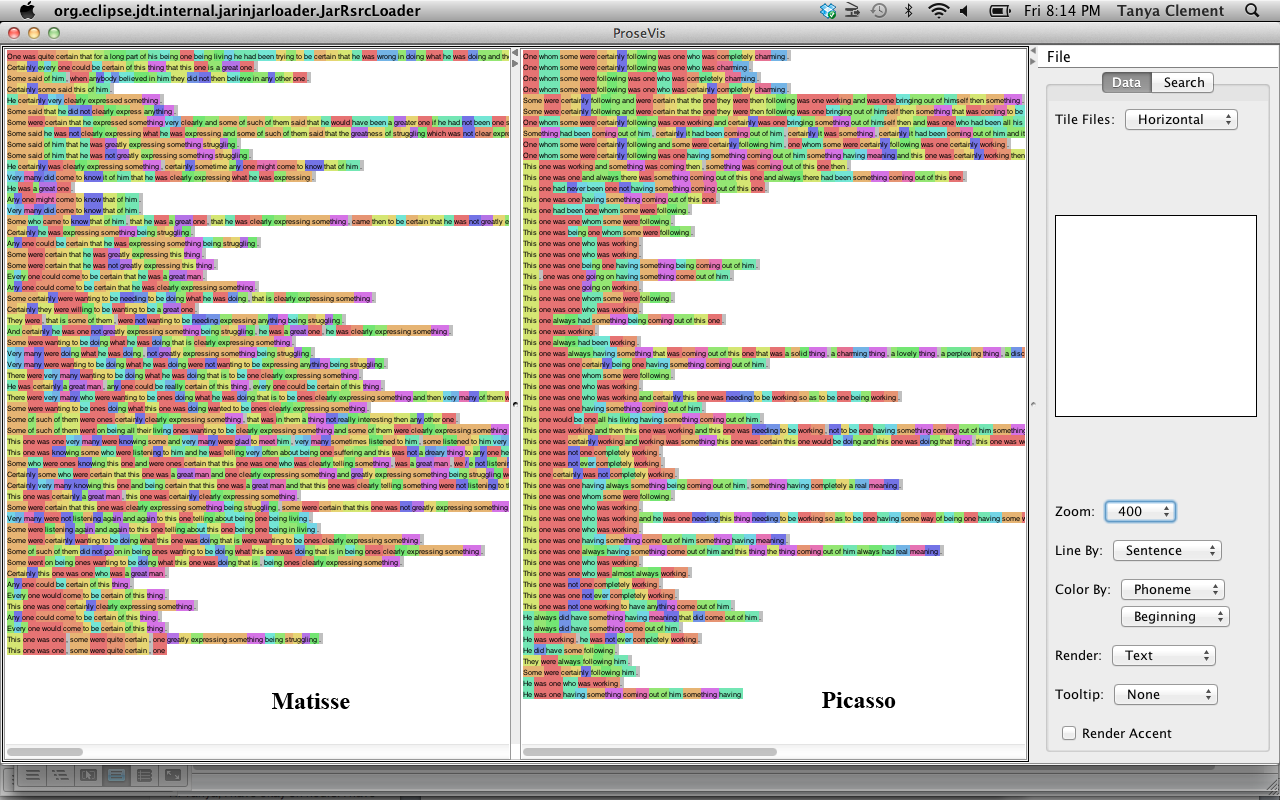
\includegraphics[scale=0.24]{../img/prosevis.png}
	\caption{Comparison of two poems in ProseVis.\protect\footnote{https://sourceforge.net/projects/prosevis/}}\label{screenshotProsevis}
\end{figure}

\subsection{Poemage and RhymeDesign}
Poemage (\cite{McCurdy2015poemage}) and RhymeDesign (\cite{McCurdy2015}) are both open-source applications with focus on analysis of sonic devices and sonic topology in poetry. Poemage focuses on complex structures of words connected through some sonic or linguistic resemblance across the space of the poem \footnote{http://www.sci.utah.edu/~nmccurdy/Poemage/}. It is available for MacOS or Windows with a web version currently under development. In MacOS application RhymeDesign - which also provides the backend for Poemage - user can enter their poem and query for one of the default rhyme types or choose a custom rhyme type.

\begin{figure}[h]\centering
	\includegraphics[scale=0.24]{../img/poemage.pdf}
	\caption{An example analysis in Poemage.}\label{screenshotPoemage}
\end{figure}

\subsection{Ambiances}
This software is unique in the fact that the analysis is integrated in the process of writing. As described in the paper \cite{Meneses2015}, writers enter the poem, receive a visualization and can control this visualization with body and hand gestures which in turn influence the poem. By such interconnection author aims to make Ambiances a part of the writing process and give it a chance to influence the final result. However the actual software does not seem to be openly available.


\section{Generation tools}
\cite{lau2018deep} - learns rhyme automatically, for sonnets, results indistinguishable, apart from expert evaluation, missing emotion